\documentclass[conference]{IEEEtran}
\usepackage[utf8]{inputenc}
\usepackage{cite}
\usepackage{tabularx} % Required for the table
\usepackage{array}    % Required for custom column types
\usepackage{longtable}
\usepackage{booktabs}
\usepackage{adjustbox} % To allow scaling of tables
\usepackage{caption}
\usepackage{stfloats}
\usepackage{authblk}
\usepackage{algorithm}      % For algorithm environment
\usepackage{algpseudocode}  % For algorithmicx commands

\begin{document}

\title{Power, Area and Thermal Prediction in 3D Network-on-Chip using Machine Learning}

\author{Abhijith C, Anand M K \\

Department of Computer Science and Engineering \\ 
	National Institute of Technology Karnataka (NITK) \\ 
	Surathkal, India\\
Email: \{abhijithc.242cs003, anandmk.242cs008\}@nitk.edu.in}


\maketitle

\section{Proposed Methodology}

Machine learning (ML) algorithms are widely used in various real-time predictions, such as energy consumption prediction and weather forecasting. The Power, Area, and Temperature (PAT) prediction of Network-on-Chip can also leverage the ability of machine learning models. However, the lack of availability of a proper public dataset is a crucial issue. In addition, most existing studies focus on power, area, or thermal analysis independently. Frameworks involving simultaneous analysis of all three parameters are rare in current research.

This work proposes a hybrid model that combines ML and DL algorithms. The ML component of the hybrid model uses algorithms such as linear regression and decision trees to predict area and power, which have a linear relationship with NoC parameters. The DL component of the model uses convolutional neural networks (CNNs) that learn complex non-linear relationships in NoC to predict temperature. The algorithms can predict PAT values for unseen input NoC configuration based on their learning. The prediction of both models is combined to produce a single output in the hybrid model.

\subsection{Linear Regression}

Linear regression is an ML algorithm that is used for predictions involving numerics. It learns the relationship between a dependent variable, the output and independent variables, the inputs, by fitting a linear equation. The equation is represented as:

\[
Y = \beta_0 + \beta_1 X_1 + \beta_2 X_2 + \dots + \beta_n X_n + \epsilon
\]

where \( Y \) is the predicted output, \( X_1, X_2, \dots, X_n \) are the input features, \( \beta_0 \) is the intercept, \( \beta_1, \beta_2, \dots, \beta_n \) are the coefficients, and \( \epsilon \) is the error term. The coefficients of the equation are learned using Mean Squared Error (MSE), a loss function. In power, area, and thermal (PAT) prediction for networks-on-chip (NoC), linear regression can predict these metrics based on input parameters such as topology size, packet injection rate, etc. However, linear regression can only learn linear relationships between the input and output variables. Therefore, methods such as decision trees are needed to learn the complex and non-linear relationships that are present in NoC systems.

\subsection{Decision Trees}

Decision trees are powerful ML algorithms used for regression and classification tasks. These algorithms split the training dataset based on the most significant feature that separates the data most precisely. The internal nodes of the decision tree define the decision on an input feature, and the leaf node represents the predicted output value. Decision trees can find complex relationships between input and output variables as they are non-parametric. In power, area, and thermal prediction in NoC systems, these algorithms can learn complex relationships between NoC parameters. Decision trees also provide a visual structure that helps researchers understand which features impact the outputs most. However, these algorithms can result in an overfitted model with  increased generalization error. Generalization error can be reduced using techniques like pruning, making these algorithms perform well in large-scale NoC systems.

\subsection{Convolutional Neural Networks}

Convolutional Neural Networks (CNNs) are DL algorithms that are widely used for tasks such as Image processing and Object detection. They extract features from the input dataset by applying filters using convolutional layers, making CNN the best algorithm for learning data structured in grid-like topologies, such as NoC systems. In power, area, and thermal prediction in the NoC system, CNNs can be used to understand non-linear relationships required for temperature prediction. CNNs work well with large datasets and can learn complex patterns in NoC designs that may not be possible for simpler algorithms like linear regression and decision trees.

\subsection{Dataset Creation}

The dataset generation process for power, area, and thermal prediction in NoC systems involves using different parameters specified in Table \ref{tab:noc_params} to generate different configurations for a NoC system. The different NoC parameters include topology, routing algorithm, network size, traffic pattern, buffer size, packet size, and packet injection rates (PIR) across the X, Y, and Z axes. The dataset is created by changing the value of the parameters to generate different configurations for an NOC system.

The dataset creation is described in Algorithm \ref{algo}. Step 1 involves generating different configurations of a NoC system by looping through different parameter values. Step 2 involves using a PAT-noxim simulator to simulate the different configurations generated in Step 1 and collecting output metrics such as total power consumption, total area, and average temperature for each configuration. Steps 3 and 4 involve storing the output metrics along with the configurations of the NoC system into a file such as a CSV file. This file will then be used to train the ML and DL models. 

\begin{table}[h!]
\centering
\begin{adjustbox}{max width=\textwidth}
\begin{tabular}{|c|c|}
\hline
\textbf{NoC Parameter} & \textbf{Parameter Values} \\
\hline
\textbf{Topology} & 3D Mesh Topology \\
\hline
\textbf{Routing Algorithm} & XYZ Routing \\
\hline
\textbf{Network Size} & 
\begin{tabular}[c]{@{}c@{}}
2x2x2, \\
3x3x3, \\
4x4x4, \\
5x5x5, \\
6x6x6, \\
7x7x7, \\
8x8x8, \\
9x9x9, \\
10x10x10, \\
12x12x12 
\end{tabular} \\
\hline
\textbf{Traffic Pattern} & 
\begin{tabular}[c]{@{}c@{}}
Random \\ 
\end{tabular} \\
\hline
\textbf{Buffer Size} & 8 \\
\hline
\textbf{Packet Size} & 16 flits \\
\hline
\textbf{Packet Injection Rate (PIR)} & \textbf{X-axis PIR}:
\begin{tabular}[c]{@{}c@{}}
[0.01, 0.05, 0.1, 0.15, 0.2]
\end{tabular} \\
& \textbf{Y-axis PIR}:
\begin{tabular}[c]{@{}c@{}}
[0.01, 0.05, 0.1, 0.15, 0.2]
\end{tabular} \\
& \textbf{Z-axis PIR}:
\begin{tabular}[c]{@{}c@{}}
[0.0001, 0.001, 0.005, 0.01]
\end{tabular} \\
\hline
\textbf{Sample Period} & 20000000 \\
\hline
\end{tabular}
\end{adjustbox}
\caption{NoC Parameters and Values}
\label{tab:noc_params}
\end{table}

\begin{algorithm}[h]
\caption{Generate Data Points for NoC Dataset}
\label{algo}
\begin{algorithmic}[1]
    \State \textbf{Input:} Set of NoC parameters:
        \begin{itemize}
            \item \textbf{Topologies}: \{2x2x2, 3x3x3, 4x4x4, 5x5x5, 6x6x6, 7x7x7, 8x8x8, 9x9x9, 10x10x10, 12x12x12\}
            \item \textbf{Traffic Patterns}: \{Random\}
            \item \textbf{Buffer Size}: 8 flits
            \item \textbf{Packet Size}: 16 flits
            \item \textbf{PIR Values}:
                \begin{itemize}
                    \item X-axis PIR: \{0.01, 0.05, 0.1, 0.15, 0.2\}
                    \item Y-axis PIR: \{0.01, 0.05, 0.1, 0.15, 0.2\}
                    \item Z-axis PIR: \{0.0001, 0.001, 0.005, 0.01\}
                \end{itemize}
            \item \textbf{Sample Period}: 20,000,000 cycles
        \end{itemize}
        
    \State \textbf{Step 1: Generate Configurations}
    \For {each topology in Topologies}
        \For {each traffic pattern in Traffic Patterns}
            \For {each PIR\_x in X-axis PIR}
                \For {each PIR\_y in Y-axis PIR}
                    \For {each PIR\_z in Z-axis PIR}
                        \State Create a configuration with the parameters: \{topology, traffic pattern, PIR\_x, PIR\_y, PIR\_z, buffer size, packet size, sample period\}
                    \EndFor
                \EndFor
            \EndFor
        \EndFor
    \EndFor
    
    \State \textbf{Step 2: Simulate and Gather Metrics}
    \For {each configuration generated}
        \State Run the simulation to gather metrics: \{total power, total area, average temperature\}
    \EndFor
    
    \State \textbf{Step 3: Store Results}
    \For {each configuration}
        \State Store the configuration parameters and the gathered metrics
    \EndFor
    
    \State \textbf{Step 4: Save Dataset}
    \State Save the dataset with the 1000 configurations and metrics to a file (e.g., CSV)
    
\end{algorithmic}
\end{algorithm}

\subsection{Design of Proposed Method}
Algorithm 2 describes the flow of the proposed method. Step One involves dataset generation using the PAT-Noxim simulator, as described in Algorithm 1. The dataset is normalized to ensure that all the parameters equally contribute to the ML prediction. The duplicate data is removed to ensure the proposed model is trained on different data. The dataset is split into training (70\%), testing (15\%), and validation (15\%).

The proposed hybrid model includes ML components for Power and Area prediction and DL components for Temperature prediction. The training of the linear regression model minimizes the MSE between the predicted and actual values of power and area. 

\[
MSE = \frac{1}{n} \sum_{i=1}^{n} \left( Y_i - \hat{Y_i} \right)^2
\]

Where:
\begin{itemize}
    \item \( Y_i \): Actual output
    \item \( \hat{Y_i} \): Predicted output
    \item \( n \): Number of samples
\end{itemize}
The ability of the model to predict power and area on unseen NoC configurations are evaluated using the MSE.
The dataset is also trained on a decision tree algorithm to predict the power and area. This training phase involves splitting the dataset based on the most significant feature that separates the data most precisely. The MSE is used to calculate the ability of the model to predict accurately. 

The CNN model is designed to train the dataset for temperature prediction. The architecture consists of the following layers:

\begin{itemize}
	\item \textbf{Input Layer}: Accepts the input parameters.
	
	\item \textbf{Convolutional Layer 1}: Applies a set of convolutional operations to extract features from input. ReLU is used as an activation function.
	\begin{itemize}
		\item ReLU returns the maximum of 0, and the input value introduces non-linearity in the model. It can be represented as:
		\[
		f(x) = \max(0, x)
		\]
	\end{itemize}
	
	\item \textbf{Max-Pooling Layer}: Reduces the size of the feature map without losing extracted information.  
	
	\item \textbf{Convolutional Layer 2}: Extracts more features from the pooled feature map.
	
	\item \textbf{Flattening Layer}: Converts the feature map to a single-dimensional vector.
	
	\item \textbf{Fully Connected Layer}: Aggregates the learned features.
	
	\item \textbf{Output Layer}: Outputs the predicted thermal value with a linear activation function. The linear function output is the same as the input. It can be represented as:
	\[
	f(x) = x
	\]
\end{itemize}
The predicted power area and temperature are combined, and the model is tested using a test dataset. The flowchart of the proposed method is given in Fig. 1.


\begin{algorithm}
\caption{Algorithm for Proposed Framework}\label{alg:pat_prediction}
\begin{algorithmic}[1]
    \State \textbf{Input:} Set of NoC parameters: Topology, Traffic Pattern, PIR (X, Y, Z), Buffer Size, Packet Size, Sample Period
    \State \textbf{Output:} Predicted values of Power, Area, and Temperature
    
    \State \textbf{Step 1: Dataset Creation}
    \State Create dataset using simulation tool (PAT Noxim) based on input NoC parameters
    \State Extract Power, Area, and Temperature as output labels
    
    \State \textbf{Step 2: Data Preprocessing}
    \State Normalize or scale the dataset
    
    \State \textbf{Step 3: Train-Test Split}
    \State Split the dataset into Training, Validation, and Test sets (e.g., 70\% training, 15\% validation, 15\% testing)
    
    \State \textbf{Step 4: Model Training}
    \State \textbf{ML Component:}
    \State Train a \textbf{Linear Regression} model for Power and Area prediction
    \State Train a \textbf{Decision Tree} model for Power and Area prediction
    
    \State \textbf{DL Component:}
    \State Train a \textbf{CNN} for Temperature prediction
    
    \State \textbf{Step 5: Model Evaluation}
    \State Use validation data to evaluate both models
    
    \State \textbf{Step 6: Combine Predictions}
    \State Combine the outputs from the ML and DL models for final Power, Area, and Temperature predictions
    
    \State \textbf{Step 7: Testing and Final Prediction}
    \State Test the combined model on the test set and make the final prediction
    
    \State \textbf{End}
\end{algorithmic}
\end{algorithm}

\begin{figure}[h]  % Begin the figure environment
    \centering
    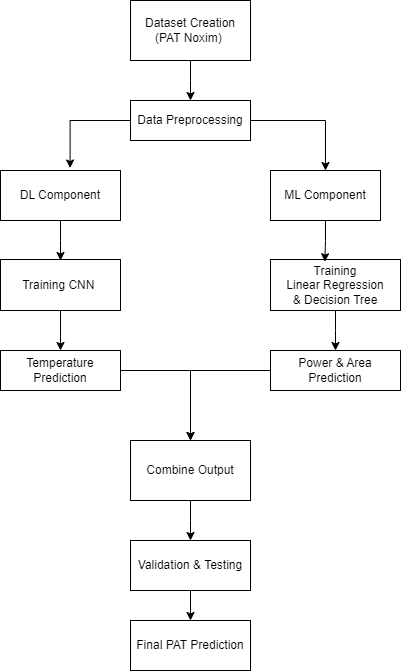
\includegraphics[width=0.8\linewidth]{Proposed.png}  % Specify the path to your image
    \caption{Illustration of the Proposed Framework}  % Add a caption for the image
    \label{fig:proposed_framework}  % Add a label for referencing the image
\end{figure}

\subsection*{Conclusion}

This work proposes a hybrid model that combines ML and DL algorithms. The ML component uses linear regression and decision trees to predict area and power, and the DL component uses CNN to predict temperature. The dataset is generated using PAT-noxim with different NoC parameters. The trained model is evaluated with unseen data, and prediction accuracy is calculated.  






\end{document}
